\documentclass[12pt]{article}
\usepackage{amssymb, amsmath, amsfonts, bm, graphicx, geometry}
\usepackage{tabularx, booktabs, float, enumitem, multicol, mathtools,mathrsfs}
\geometry{margin=1in}


\title{}
\date{}
\author{}

\begin{document}

\begin{titlepage}
    \centering
    \vspace*{1in}

    % Title of the experiment and identifying number
    {\Large\bfseries Lab 4: RC Circuit Response to Square Wave Voltage Input \par}
    \vspace{1.5cm}

    % Course number
    {\large ESC 221 Basic Principles of Electrical Engineering \par}
    \vspace{2cm}

    % Author's name
    {\large \textbf{Author:} Zeshui Song \par}
    \vspace{0.5cm}

    % Names of other lab group members
    {\large \textbf{Lab Partners:}} \\
    Roy He, Phillip Joseph, Bella Im, and Kieran Cheng
    \vfill

    % Date on which the lab was performed
    {\large Date Performed: April 16, 2026 \par}
    \vspace{0.8cm}

    % Name of organization sponsoring the work
    {\large Cooper Union \par}

    \vspace*{1in}
\end{titlepage}
\newpage

\section*{I. Introduction, Experimental Method and Hypotheses}
\textbf{A. Introduction}\\\\
This experiment investigates the time domain response of a series resistor-capacitor (RC) circuit to a square wave voltage input. The objective is to observe the charging and discharging voltage behavior across the capacitor, and analyze the relationship between the time constant of the circuit and its ability to reach a steady state value given varying input frequencies.\\\\
\textbf{B. Experimental Method}\\\\
In the series RC circuit constructed as shown in Figure \ref{fig:Circuit}, the function generator produces a square-wave input voltage with an amplitude of 5 V and periods of 8$\tau$ and 2$\tau$, where $\tau$ is the circuit time constant. The voltage across the capacitor is measured on an oscilloscope alongside the Transistor-Transistor Logic (TTL) output of the function generator. By varying the input voltage frequency, the charging and discharging behavior of the capacitor can be observed.\\\\
Note that the TTL output of the function generator is synchronized in time with the actual voltage output, but is limited to 5 V and inverted in polarity when displayed on the oscilloscope.
\newpage\noindent
\textbf{C. Hypotheses}\\\\
It is predicted that the capacitor will follow an exponential charging and discharging curve defined by the time constant $\tau = R_1C_1$. The time domain response of the voltage is derived in the Appendix for each period of the square wave input voltage, and is given by:
\[\boxed{v_C(t) =
\begin{cases}
v_m\left(1 - e^{-t/\tau}\right), & t < T/2 \quad \text{(charging)}\\
v_me^{-t/\tau}\left(e^{\frac{T}{2\tau}}-1\right), & t \ge T/2\quad \text{(discharging)}
\end{cases}}\]
Thus, it is expected that when the period of the input voltage is much larger than the time constant ($T \gg \tau$), the capacitor will have sufficient time to charge and discharge fully, reaching a steady state value of $v_m$ during the charging phase and 0 V during the discharging phase. However, when the period of the input voltage is comparable to the time constant ($T \approx \tau$), the capacitor will not have sufficient time to charge and discharge fully, resulting in a voltage response that does not reach the steady state values of $v_m$ and 0 V, but rather oscillates between intermediate values.\\\\
Where the theoretical time constant is calculated to be 
\[\tau = R_1C_1 = [1 \times10^3\,\Omega]\cdot[2\times10^{-6} \,\text{F}] = 2 \times 10^{-3} \, \text{s}\]
The theoretical voltage response of the capacitor is plotted below in Figures \ref{fig:4tau}, \ref{fig:comparison}, and \ref{fig:squarewave}:
\begin{figure}[H]
    \centering
    
\includegraphics[width=1\linewidth]{Figure_1.png}
    \caption{Theoretical capacitor voltage response to a step voltage input with period 8$\tau$, shown alongside the voltage input waveform and time constant ($\tau$) for reference. With the input turned on for $4\tau$, the capacitor is expected to reach approximately 98.2\% of its steady-state voltage during each charging interval.}
    \label{fig:4tau}
\end{figure}
\begin{figure}[H]
    \centering
    
\includegraphics[width=1\linewidth]{Figure_2.png}
    \caption{Comparison of theoretical capacitor voltage responses to step voltage inputs with periods of 2$\tau$ through 10$\tau$ (pulse durations of 1$\tau$ to 5$\tau$). The cases with 1$\tau$ and 4$\tau$ pulse durations are highlighted for comparison with experimental results. As the pulse duration increases, the capacitor voltage response approaches the steady-state value of $v_m$ according to the exponential charging curve.}
    \label{fig:comparison}
\end{figure}
\begin{figure}[H]
    \centering
    
\includegraphics[width=1\linewidth]{Figure_3.png}
    \caption{Comparison of theoretical capacitor voltage responses to square wave of varying periods (2$\tau$ and 8$\tau$), with the voltage input waveform and time constant ($\tau$) for reference.}
    \label{fig:squarewave}
\end{figure}
\newpage
\section*{II. Equipment List}
\begin{enumerate}
    \item \textbf{Function Generator} \\ 
          Manufacturer: GW Instek \\
          Model: SFG-1003
    \item \textbf{Oscilloscope} \\ 
          Manufacturer: GW Instek \\
          Model: GDS-820C
\end{enumerate}
\newpage
\section*{III. Wiring / Schematic Diagram / Procedure}
\textbf{A. Procedure}\\\\
1. Calculating Circuit Parameters
\begin{enumerate}
    \item The time constant was calculated to be 
    \[\tau = R_1C_1 = [1 \times10^3\,\Omega]\cdot[2\times10^{-6} \,\text{F}] = 2 \times 10^{-3} \, \text{s}\]
    \item For a period of 8$\tau$, the frequency of the square wave input voltage was calculated to be
    \[f_{8\tau} = \frac{1}{T} = \frac{1}{8\tau} = \frac{1}{8\cdot [2 \times 10^{-3} \, \text{s}]} = 62.5 \, \text{Hz}\]
    \item For a period of 2$\tau$, the frequency of the square wave input voltage was calculated to be
    \[f_{2\tau} =4f_{8\tau} = \frac{1}{2\tau} = \frac{1}{2\cdot [2 \times 10^{-3} \, \text{s}]} = 250 \, \text{Hz}\]
\end{enumerate}
2. Constructing the Circuit
\begin{enumerate}
    \item The circuit was constructed as shown in Figure \ref{fig:Circuit}, with two 1 $\mu$F capacitors wired in parallel to achieve the desired capacitance of 2 $\mu$F, and a 1 k$\Omega$ resistor. 
    \item The function generator output was set to a 5V square with the calculated frequency of 62.5 Hz for the 8$\tau$ case, and 250 Hz for the 2$\tau$ case.
\end{enumerate}
3. Measurement and Data Collection
\begin{enumerate}
    \item Channel 1 of the oscilloscope was connected to the TTL output of the function generator.
    \item Channel 2 of the oscilloscope was connected across the capacitor at nodes A and B to measure the voltage response.
    \item Starting with the function generator set to 62.5 Hz ($T = 8\tau$), the voltage response across the capacitor was observed and recorded on the oscilloscope.
    \item The frequency of the function generator was then changed to 250 Hz ($T = 2\tau$), and the voltage response across the capacitor was again observed and recorded on the oscilloscope.
\end{enumerate}
\newpage\noindent
\textbf{B. Schematic Diagram}
\begin{figure}[H]
    \centering
    
\includegraphics[width=0.6\linewidth]{Circuit.png}
    \caption{A series RC circuit consisting of a resistor and capacitor in series with a square wave voltage input source. Nodes A and B are the measurement points for the voltage across the capacitor.}
    \label{fig:Circuit}
\end{figure}
\newpage
\section*{IV. Results}
\textbf{Input: $f=62.5$ Hz, $T=8\tau$, Pulse Duration = $4\tau$}
\begin{figure}[H]
    \centering
    
\includegraphics[width=0.6\linewidth]{1.png}
    \caption{Oscilloscope reading showing a peak capacitor voltage of 5.76V, indicating that the input voltage was miscalibrated and is approximately 5.76V rather than the expected 5V.}
    \label{fig:exp1}
\end{figure}
\begin{figure}[H]
    \centering
    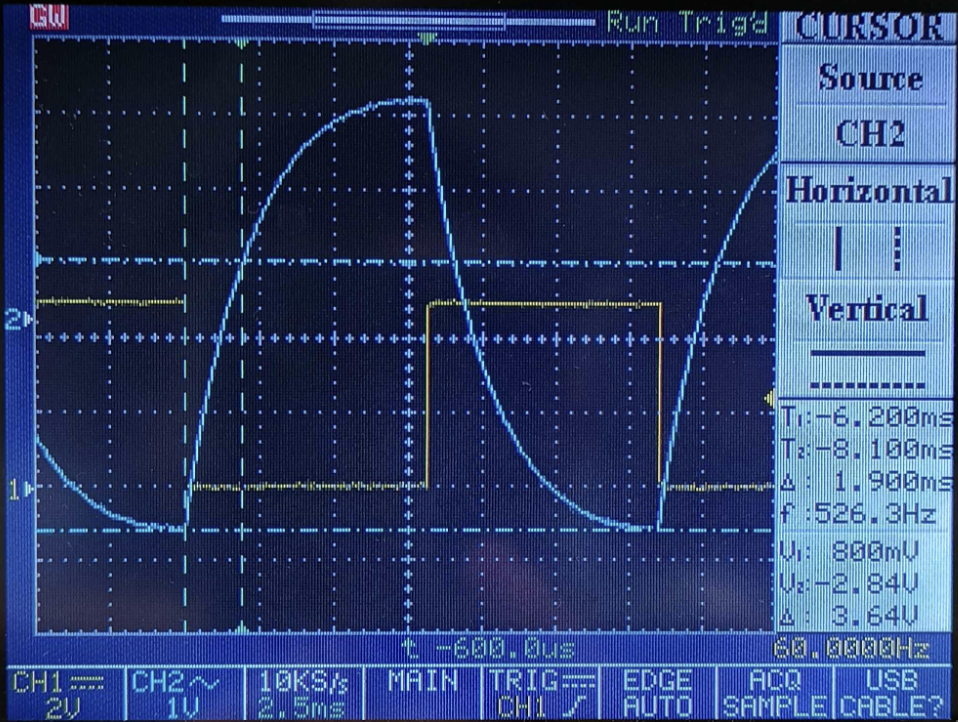
\includegraphics[width=0.6\linewidth]{1-1.png}
    \caption{The experimental time constant $\tau$ was found to be 1.9 ms, at the point where the capacitor voltage reached approximately 63.2\% of its steady-state value ($0.63\cdot[5.76\,\text{V}]$).}
    \label{fig:exp1-1}
\end{figure}
\newpage\noindent
\textbf{Input: $f=250$ Hz, $T=2\tau$, Pulse Duration = $\tau$}
\begin{figure}[H]
    \centering
    
\includegraphics[width=0.6\linewidth]{2.png}
    \caption{Oscilloscope reading of the peak voltage across the capacitor for the 2$\tau$ case to be 2.6V. Note that the minimum voltage for this case is not 0V, as the capacitor does not have sufficient time to fully discharge before the next charging interval begins.}
    \label{fig:exp2}
\end{figure}
\noindent
\textbf{Summary of Results}
\begin{table}[h!]
\centering
\caption{Comparison of Calculated and Experimental RC Circuit Parameters}
\label{table:results_summary}
\begin{tabular}{|l|c|c|}
\hline
\textbf{Parameter} & \textbf{Theoretical Value} & \textbf{Experimental Value} \\ \hline
Time Constant ($\tau$) & 2.0 ms & 1.9 ms \\ \hline
Input Voltage ($V_m$) & 5.0 V & $\approx$ 5.76 V \\ \hline
Peak $V_C$ ($T=8\tau$) & $\approx$ 5.0 V & 5.76 V \\ \hline
$\Delta V_C$ ($T=2\tau$) & 2 V* & 2.6 V \\ \hline
\end{tabular}
\end{table}\\
*Calculated in the Appendix. Note that if using the actual input voltage of 5.76 V rather than the expected 5 V, the predicted $\Delta v_C$ for the 2$\tau$ case is approximately 2.304V rather than 2V.
\newpage
\section*{V. Discussion, Analysis and Concluding Statements}
\textbf{A. Observations on the output signal following a change in the input signal}\\
Following a change in the input signal, the output signal across the capacitor exhibited an exponential charging and discharging behavior, as predicted by the theoretical analysis. The change is not instantaneous and is governed by the time constant $\tau$ of the circuit, which determines how quickly the capacitor charges and discharges in response to changes in the input voltage.\\\\
\textbf{B. Steady state behavior at varying frequencies}\\
As shown in Figure \ref{fig:exp1}, at the lower frequency of 62.5 Hz (period of 8$\tau$), the capacitor was able to get close to steady state (within 98.2\%) because the pulse duration of 4$\tau$ allowed the capacitor to fully charge and discharge per cycle. However, as shown in Figure \ref{fig:exp2}, at the higher frequency of 250 Hz (period of 2$\tau$), the capacitor did not have sufficient time to fully charge and discharge, resulting in a max and min voltage that does not reach the steady state values of $v_m$ and 0 V.\\\\
\textbf{C. Relationship between steady state and RC time constant}\\
The time constant governs how quickly the circuit responds to changes to the input voltage and thus how quickly it can reach steady state as shown in Figure \ref{fig:exp1-1}. A shorter time constant will allow the circuit to reach steady state in a shorter amount of time, while a longer time constant will result in a slower response and a longer time to reach steady state.\\\\
\textbf{D. Relationship between steady state and input frequency}\\
The input frequency must match the time constant of the circuit in order for the circuit to reach steady state. If the input frequency is too high (period too short), the circuit will not have sufficient time to reach steady state before the next change in input voltage occurs. On the other hand, a low input frequency (long period) allows the circuit to reach steady state before the next change in input voltage occurs.\\\\
\textbf{E. Conclusion}\\
This experiment successfully verified the time-domain response of a series RC circuit to a square wave voltage input. While there were small discrepancies between the theoretical and experimental values for the voltage response of the capacitor, the general trends and behavior of the circuit were consistent with theoretical models.\\\\
One source of error is that the input voltage did not behave as an ideal step. Instead, it exhibited a finite rise with a slight slope and curvature before reaching its maximum amplitude $v_m$, which likely introduced a small delay in the circuit's response. Additionally, the function generator has an internal resistance of 50 $\Omega$, which forms a voltage divider with the 1 k$\Omega$ circuit resistance. As a result, the circuit receives about 95\% of the set output voltage, leading to a slightly reduced input compared to the expected value.
\newpage
\section*{VI. Appendix}
\textbf{Calculation for Predicted Voltage Response}
\begin{center}
    
\includegraphics[width=0.6\linewidth]{Circuit.png}
\end{center}
Defining the following parameters:
\begin{itemize}
    \item $v_m$: Amplitude of the square wave input voltage
    \item $T$: Period of the square wave input voltage
\end{itemize}
The function generator has a duty cycle of 50\%, meaning that it is on for half of each period ($T/2$). Thus, one period of the square wave input voltage can be defined using the Heaviside step function $\mathscr{U}(t-a)$ as follows:
\[v_\text{in}(t)=v_m(1-\mathscr{U}(t-T/2))\]
Such that
\[v_{\text{in}}(t) = 
\begin{cases} 
v_m, & t < T/2 \\
0, & t \ge T/2 
\end{cases}\]
Deriving the governing equation for the voltage across the capacitor $v_C(t)$ using KCL at node A, using node B as the reference node:
\[\frac{v_\text{in}-v_a}{R_1} = C_1\frac{dv_a}{dt}\]
Since $v_a = v_C$, the governing equation can be rewritten as:
\[R_1C_1\frac{dv_C}{dt} + v_C = v_m(1-\mathscr{U}(t-T/2))\]
\underline{Finding $v_C(t)$}\\
Letting $\tau = R_1C_1$, the governing equation can be rewritten as:
\[\tau\frac{dv_C}{dt} + v_C = v_m(1-\mathscr{U}(t-T/2))\]
Taking the Laplace transform, assuming zero initial conditions:
\[\tau sV_C(s) + V_C(s) = v_m\left(\frac{1}{s} - \frac{e^{-\frac{T}{2}s}}{s}\right)\]
\[V_C(s) \left(\tau s + 1\right) = v_m \left(\frac{1-e^{-\frac{T}{2}s}}{s}\right)\]
\[V_C(s) = v_m(1-e^{-\frac{T}{2}s})\left(\frac{1}{s(\tau s + 1)}\right)=v_m(1-e^{-\frac{T}{2}s})\left(\frac{1/\tau}{s(s + 1/\tau)}\right)\]
Partial fraction decomposition:
\[\frac{1/\tau}{s(s + 1/\tau)} = \frac{A}{s} + \frac{B}{s + 1/\tau}\]
Using the limit method to solve for $A$ and $B$:
\[A = \lim_{s\to 0} \left(s\frac{1/\tau}{s(s + 1/\tau)} \right)= 1\]
\[B = \lim_{s\to -1/\tau} \left((s + 1/\tau)\frac{1/\tau}{s(s + 1/\tau)} \right)= -1\]
Thus, the partial fraction decomposition can be rewritten as:
\[\frac{1/\tau}{s(s + 1/\tau)} = \frac{1}{s} - \frac{1}{s + 1/\tau}\]
Plugging this back into the expression for $V_C(s)$:
\[V_C(s) = v_m(1-e^{-\frac{T}{2}s})\left(\frac{1}{s} - \frac{1}{s + 1/\tau}\right)\]
\[V_C(s) = v_m\left(\frac{1}{s} - \frac{1}{s + 1/\tau}\right)-v_m e^{-\frac{T}{2}s}\left(\frac{1}{s} - \frac{1}{s + 1/\tau}\right)\]
Taking the inverse Laplace transform:
\[v_C(t) = v_m\left(1 - e^{-t/\tau}\right) - v_m \mathscr{U}(t-T/2)\left(1 - e^{-\left(t-\frac{T}{2}\right)/\tau}\right)\]
\[\boxed{v_C(t) =
\begin{cases}
v_m\left(1 - e^{-t/\tau}\right), & t < T/2 \quad \text{(charging)}\\
v_me^{-t/\tau}\left(e^{\frac{T}{2\tau}}-1\right), & t \ge T/2\quad \text{(discharging)}
\end{cases}}\]
\newpage\noindent
\textbf{Calculation for $\Delta v_C$}\\
Input: $v_m = 5$ V, $f=250$ Hz, $T=2\tau$, Pulse Duration = $\tau$\\\\
Max voltage is at $t=T/2 = \tau$:
\[v_C(\tau) = v_m\left(1 - e^{-\tau/\tau}\right) = v_m\left(1 - e^{-1}\right) \approx 0.63v_m\]
Minimum voltage is at $t=T = 2\tau$:
\[v_C(2\tau) = v_me^{-2\tau/\tau}\left(e^{\frac{2\tau}{2\tau}}-1\right) = v_me^{-2}\left(e^{1}-1\right) \approx 0.23v_m\]
Thus, the change in voltage across the capacitor is calculated to be:
\[\Delta v_C = v_C(\tau) - v_C(2\tau) \approx 0.63v_m - 0.23v_m = 0.40v_m = 2 \, \text{V}\]
Note that since the input voltage was miscalibrated to be approximately 5.76V rather than the expected 5 V, the predicted $\Delta v_C$ for the 2$\tau$ case is approximately 2.304V rather than 2V.
\end{document}